\documentclass[12pt]{article}
\usepackage{geometry}
\usepackage{booktabs}  % for \toprule style rules}
\usepackage{amsmath, amssymb}
\usepackage{algorithm}
\usepackage{algorithmic}
\usepackage{float} 
\usepackage{graphicx}
\usepackage{amsthm}
\usepackage[style=ieee]{biblatex}
\addbibresource{references.bib}
\geometry{a4paper, margin=2.5cm}

\newtheorem{theorem}{Theorem}[section]
\newtheorem{lemma}[theorem]{Lemma}
\newtheorem{corollary}[theorem]{Corollary}
\newtheorem{remark}[theorem]{Remark}

\begin{document}



\begin{titlepage}
    \centering
    
    \vspace*{2cm}
    
    % Top rule
    \noindent\rule{\linewidth}{0.8pt}
    
    \vspace{0.5cm}
    
    % Title
    {\large\textbf{SCDL3991: Regret Bound Analysis of Multi-Armed Bandit Problems}}
    
    \vspace{0.5cm}
    
    % Bottom rule
    \noindent\rule{\linewidth}{0.8pt}
    
    \vspace{4cm}
    
    % Author info
    Author: Robert Zhang \\
    SID: 540858851
    
    \vspace{3cm}
    
    % University name in small caps
    {\large\textsc{The University of Sydney}}
    
    \vspace{1.5cm}
    
    % Date
    June 15 2026
    
\end{titlepage}

\setcounter{page}{1}  % restart numbering
\tableofcontents
\newpage

\section{Introduction}

\subsection{Background}

Multi-armed bandits is a simple yet powerful framework of algorithms that make sequential decisions under uncertainty, where an agent repeatedly selects from a set of actions ("arms") and observes only the reward of the chosen action. The concept of multi-armed bandits has been studied since the 1930s, but its formal mathematical model was not established until the 1950s,  initially applied to clinical trials by the Center for Drug Evaluation and Research with the aim of identifying the most effective treatment \cite{article1}. The core objective in this situation is to maximise cumulative rewards over a finite time horizon, despite not knowing which arm is the best in advance. This problem setting captures the fundamental trade-off between exploration and exploitation: the need to learn about uncertain arms while also being able to simultaneously exploit currently known information. 

\subsection{Motivation}

Many real-world systems require making sequential decisions under uncertainty such as: online advertising, clinical trials, recommender systems etc \cite{article2}. In these settings, the decision-maker does not have prior knowledge of the reward distributions associated with each action, and must learn these distributions through interaction over time. Feedback is only available for actions that are taken, meaning that information gathered is inherently partial and must be gathered sequentially. As a result, naive strategies that focus only on immediate reward often perform poorly in the long run, while purely exploratory strategies are inefficient and costly. This highlights the need for systematic strategies that balance exploring less-known actions and exploiting currently estimated best actions. The multi-armed bandit framework provides a formal way to study this trade-off.

\subsection{Aims}

The aim of this research project is to analyse and compare different classical bandit algorithms in terms of their ability to manage the fundamental exploration-exploitation tradeoff. This report will focus on both theoretical performance guarantees and empirical behaviour, with particular attention to regret as a measure of performance over time. 

\subsection{Roadmap}

The remainder of this report is organised with 4 sections. First, we introduce the formal problem formulation where we will define the notation of the problem by introducing terms like the reward distributions, expected rewards, and cumulative regret. Next we will take a look at the key bandit algorithms which will be analysed: uniform exploration, greedy-epsilon, successive elimination, UCB, and Thompson sampling and how to prove the upper bound of their respective performances. We will then prove a guaranteed lower bound performance for all bandit algorithms and conclude the report. Finally, simulate our algorithms on a numerical example and compare the results with their theoretical performance bounds

\section{Problem Formulation and Setup}

Consider a stochastic multi-armed bandit problem with $K$ possible actions to choose from a.k.a $arms$ which are indexed from $1, 2, \cdots K$, and $T$ rounds that we play over. Each arm $a$ is associated with an unknown reward distribution denoted by $\mathcal{D}_a$ with mean reward $\mu_a$ where $\mu(a) = \mathbb{E}[\mathcal{D}_a]$. For each round $t = 1,2,\dots,T$ a bandit algorithm only observes and collects a reward for the selected arm. The algorithm’s goal is to maximise its total reward over the $T$ rounds. 

We make three key assumptions about this model: the algorithm observes only the reward for the selected action, and nothing else. In particular, it does not observe rewards for other actions that could have been selected. The reward for each arm is assumed to be independent and identically distributed (i.i.d.). For each arm $a$ that we choose, we independently sample a reward from its reward distribution $\mathcal{D}_a$ which is unknown to the algorithm. Per-round rewards are bounded; we will enforce the restriction to the interval $[0, 1]$ for simplicity.

Thus a bandit algorithm is summarised as:

\begin{algorithm}
	\caption{Stochastic Bandits}
	\begin{algorithmic}
	\STATE \textbf{Parameters:} $K$ arms, $T$ rounds (known), reward distribution $\mathcal{D}_a$ for each arm $a$  (unknown)
	\FOR{$t = 1$ \TO $T$}
	    \STATE Choose arm $a_t$,
	    \STATE Reward $r_t \in [0, 1]$ is sampled independently from distribution $\mathcal{D}_a$, $a = a_t$
	    \STATE Algorithm collects $r_t$ and observes nothing else
	\ENDFOR
	\end{algorithmic}
\end{algorithm}

In this algorithm and subsequent bandit algorithms, we are interested in the mean reward vector $\mu \in [0,1]^K$, where $\mu(a) = \mathbb{E}[\mathcal{D}_a]$. For simplicity we will use the Bernoulli distribution to model rewards, when the reward of each reward $a$ can be either 1 or 0 ("success or failure"). The problem instance is specified by the time horizon $T$ and the mean reward vector. The best mean reward is $\mu^* := \max_{a \in A} \mu(a)$. The difference $\Delta (a) = \mu^*  - \mu(a)$ describes how bad arm $a$ is compared to $\mu^*$ ; we call the gap of arm $a$. An optimal arm is an arm $a$ with $\mu(a) = \mu^*$. We measure performance by comparing the cumulative reward to the best-arm benchmark $\mu^*  \cdot T:$  where Regret $R(T)$ is defined as: 

\begin{equation}
R(T) = \mu^* T - \sum_{t=1}^{T} \mu_{a_t}
\tag{2.1}
\label{eq:regret-formula}
\end{equation}


Note that the selected arm \(A_t\) itself is random variable, since the algorithm’s choice can depend on previously observed random rewards and may also involve randomised decision rules. Consequently, the cumulative regret $R(T)$ is also a random variable. We analyse the performance of an algorithm with regards to the dependence on the number of arms $K$ and the time horizon $T$ and use big-O notation to focus on the asymptotic dependence on the parameters of interests, rather than keep track of the constants.

\section{Methodology}

\subsection{Uniform Exploration}

The first multi-armed bandit algorithm that we will analyse is uniform exploration. The idea behind this algorithm is that we explore all arms uniformly (at the same rate), regardless of what has been observed previously, and then pick the empirically best arm for exploitation. This leads to the explore-first algorithm where we dedicate an initial amount of rounds for exploration and then the rest for exploration. This algorithm can be summarised as: 

\begin{algorithm}
\caption{Explore-First with parameter $N$}
\begin{algorithmic}[1]

\STATE \textbf{Exploration phase:} try each arm $N$ times
\STATE Select the arm $\hat{a}$ with the highest average reward (break ties arbitrarily)
\STATE \textbf{Exploitation phase:} play arm $\hat{a}$ in all remaining rounds

\end{algorithmic}
\end{algorithm}

The parameter $N$ is fixed and will be determined as a function of $K$ and $T$ so as to minimise regret. Let us now analyse the expected regret of this algorithm. Let the average reward for each action a after exploration phase be denoted $\mu(\bar{a})$. We define $\mu(\bar{a}) := \frac{1}{N} \sum_{i = 1}^{N} X_i (a)$ where $X_i (a)$ is the random variable denoting the reward you observe on the $i$-th pull of arm $a$. We have that $X_i(a) \overset{\text{i.i.d.}}{\sim} \mathcal{D}_a \quad \text{for } i = 1, \dots, N$ as each pull of arm $a$ returns an independent sample from the reward distribution $\mathcal{D}_a$. We want this empirical average reward $\mu(\bar{a})$ to be a good estimate of the true estimate rewards for each arm meaning the quantity $| \mu(\bar{a}) - \mu(a) |$ should be small. We bound it using the Hoeffding inequality \cite{Dubhashi_Panconesi_2009}:

\begin{equation}
\Pr\!\left[ \left| \bar{\mu}(a) - \mu(a) \right| \le \mathrm{rad} \right]
\ge 1 - \frac{2}{T^4},
\;\text{where }\;
\mathrm{rad} := \sqrt{\frac{2\log T}{N}}
\tag{3.1}
\label{eq:rad-bound}
\end{equation}

Thus, $\mu(a)$ lies in the confidence interval $[\, \bar{\mu}(a) - \mathrm{rad},\; \bar{\mu}(a) + \mathrm{rad} \,]$ with high probability and $\mathrm{rad}$ is the confidence radius of this interval. We define the clean event as the event that the deviation bound in \eqref{eq:rad-bound} holds for all arms simultaneously, i.e. $\mathcal{E} := \bigcap_{a=1}^K \left\{ |\hat{\mu}(a) - \mu(a)| \le \mathrm{rad} \right\}$. Using this we can ignore low-probability “bad events” in the analysis. This simplifies proofs, at the cost of slightly larger constants in asymptotic bounds.

\textbf{Proof:} for $K$ arms we want all arms to simultaneously satisfy $\forall a \in [K]: \left| \bar{\mu}(a) - \mu(a) \right| \le \mathrm{rad}$, 
and by the union bound we have $\Pr[\forall a \in [K]: |\bar{\mu}(a) - \mu(a)| \le \mathrm{rad}] \ge 1 - \frac{2K}{T^4}$. Each arm is chosen $N$ times and each round in exploration contributes trivially at most 1 to regret.  
For the exploitation phase, let the best arm be $a^*$and suppose the algorithm chooses an arm $a \neq a*$. This must have been
because its average reward was better than that of $a^*$: $\bar{\mu}(a) > \bar{\mu}(a^*).$ Since this is a clean event we have:

\[
\mu(a) + \mathrm{rad} \ge \bar{\mu}(a) > \bar{\mu}(a^*) \ge \mu(a^*) - \mathrm{rad}.
\]


\vspace{5mm}

Re-arranging the terms, it follows that $\mu(a^*) - \mu(a) \leq \mathrm{2rad}$. Thus, each round in the exploration phase contributes $\mathrm{2rad}$ to regret. We combine these contributions to get the following:

\[
R(T) \leq KN + \mathrm{2rad} \cdot T
\]

\vspace{5mm}

We then choose a $N$ that balances exploration regret $KN$ and exploitation regret. We know the per round regret  in the exploitation phase is upper-bounded by $\mathrm{2rad}$. This means we can express the regret of the exploration phase in terms of big-O notation as follows:

\[
\text{regret per round} \leq 2rad = 2 \cdot \sqrt{\frac{2\log T}{N}}
\]

\noindent In the worst case, this affects up to $T$ rounds and this gives us a big-O bound for the regret of $R_{exploit}$:

\[
R_{exploit} \leq 2T \sqrt{\frac{2\log T}{N}} 
\]

\[
R_{exploit} = O(T \mathrm{rad})  
\]

\noindent We can now express the total regret as a big-O asymptotic function (after dropping constants)

\[
R(T) = O(KN) + O(T \mathrm{rad})  = O(KN + T \sqrt{\frac{\log T}{N}}) 
\]

\noindent We can now balance the two summands inside the asymptotic formula making exploration regret $\approx$ exploitation regret and rearrange for $N$ to get:

\[
KN = T \sqrt{\frac{\log T}{N}}
\]

\noindent Solving for $N$:

\[
K N^{3/2} = T \sqrt{\log T}
\]

\[
N = \left(\frac{T}{K}\right)^{2/3} (\log T)^{1/3}
\]


\noindent Finally, substitute $N = \left(\frac{T}{K}\right)^{2/3} (\log T)^{1/3}$ to obtain:

\begin{equation}
\mathbb{E}[R(T)] = O\Big( T^{2/3} \,(K \log T)^{1/3} \Big) 
\tag{3.2}
\label{eq:regret-unf-exp}
\end{equation}

\vspace{5mm}


\begin{theorem}
Explore-first achieves regret $\mathbb{E}[R(T)] = O\Big( T^{2/3} \,(K \log T)^{1/3} \Big)$\
\end{theorem}
\begin{proof}
The probability of the bad event is at most $2/T^4$. Since the regret in any round is bounded by 1, the total regret contributed by the bad event is at most
\[
T \cdot \frac{2}{T^4} = \frac{2}{T^3},
\]
which is negligible. Therefore the expected regret is dominated by the regret on the good event, yielding
\[
\mathbb{E}[R(T)]
= O\Bigl(T^{2/3}(K\log T)^{1/3}\Bigr).
\]
\end{proof}

\newpage


\subsection{Successive Elimination}

The next multi-armed bandit algorithm that we will analyse is successive elimination. This algorithm adapts exploration to the observations so that very under-performing arms are phased out sooner. In order to do this let us introduce the idea of confidence bounds. 

Fix a round $t$ and an arm $a$, and let $n_t(a)$ be the number of rounds before $t$ in which arm $a$ is chosen, and $\bar{\mu}_t(a)$ be the average reward in those rounds. We again use the Hoeffding inequality to derive:

\begin{equation}
\Pr\!\left(\left|\bar{\mu}_t(a)-\mu(a)\right|\le r_t(a)\right)\ge 1-\frac{2}{T^4},
\qquad
r_t(a)=\sqrt{\frac{2\log T}{n_t(a)}}.
\tag{3.3}
\label{eq:confidence-bound}
\end{equation}

Since $n_t(a)$ is random, we introduce a reward tape of i.i.d. samples from $\mathcal{D}_a$ for each arm $a$. When $n_t(a)=j$, the empirical mean of arm $a$ equals $\bar v_j(a)$, the average of the first $j$ tape entries. Hence, for every fixed $j$, Hoeffding's inequality gives:

\[
\Pr\!\left(\left|\bar{v}_j(a)-\mu(a)\right|\le r_t(a)\right)\ge 1-\frac{2}{T^4}.
\]

\vspace{5mm}

Taking a union bound, it follows (assuming $K$, the number of arms, satisfies $K \le T$) that
\begin{equation}
\Pr[E] \ge 1 - \frac{2}{T^2},
\qquad
E := \left\{ \forall a\, \forall t \; \left| \bar{\mu}_t(a) - \mu(a) \right| \le r_t(a) \right\}.
\tag{3.4}
\end{equation}
The event $E$ in equation $1.4$ will be the clean event for the subsequent analysis. For each arm $a$ at round $t$, we define the upper and lower confidence bounds


\[
\mathrm{UCB}_t(a) = \bar{\mu}_t(a) + r_t(a),
\qquad
\mathrm{LCB}_t(a) = \bar{\mu}_t(a) - r_t(a).
\]
The confidence interval is $\bigl[\mathrm{LCB}_t(a), \mathrm{UCB}_t(a)\bigr]$ with confidence radius $r_t(a)$.

\noindent For $K = 2$ arms we have the algorithm:


\begin{algorithm}
\caption{Successive Elimination, $K = 2$}
\begin{algorithmic}
\STATE Alternate two arms until $\mathrm{UCB}_t(a) < \mathrm{LCB}_t(a')$ after some even round $t$.
\STATE Abandon arm $a$, and use arm $a'$ forever since.
\end{algorithmic}
\end{algorithm}

\noindent For analysis, assume the clean event. Note that the “abandoned” arm cannot be the best arm. But how much regret do we accumulate before disqualifying one arm? Let $t$ be the last round where we did not invoke the stopping rule i.e when the confidence intervals of the two arms still overlap:

\[
\Delta := |\mu(a) - \mu(a')| \le 2 \bigl( r_t(a) + r_t(a') \bigr)
\]

\noindent  Since the algorithm has been alternating the two arms before time $t$, we have $n_t(a) = \frac{t}{2}$ (up to floor and ceiling), which yields:

\[
\Delta \le 2 \bigl( r_t(a) + r_t(a') \bigr)
\le 4 \sqrt{\frac{2 \log T}{\lfloor t/2 \rfloor}}
= O\Bigl(\sqrt{\frac{\log T}{t}}\Bigr).
\]

\noindent  Then the total regret accumulated up to round $t$ is:

\[
R(t) \le \Delta \cdot t 
\le O\Bigl(t \cdot \sqrt{\frac{\log T}{t}}\Bigr)
= O\Bigl(\sqrt{t \log T}\Bigr).
\]

\vspace{5mm}

\noindent Since the probability of a bad event occuring is so small, the regret from this event is neglected hence the above expected regret.

\vspace{5mm}

\begin{lemma}
For two arms, Algorithm 1.3 achieves $\mathbb{E}[R(t)] \le O\Bigl(\sqrt{t \log T}\Bigr)$ for each round $t \le T$. 
\end{lemma}


\noindent We can extend this approach to $K > 2$ arms as follows:

\begin{algorithm}[H]
\caption{Successive Elimination for $K$ Arms}
\begin{algorithmic}[1]
\STATE \textbf{Input:} $K$ arms, horizon $T$
\STATE All arms are initially designated as active
\WHILE{there is more than one active arm}
    \STATE \textbf{new phase:} play each active arm once
    \FOR{each active arm $a$}
        \IF{$\mathrm{UCB}_t(a) < \mathrm{LCB}_t(a')$ for some other active arm $a'$} 
            \STATE Deactivate arm $a$ \COMMENT{deactivation rule}
        \ENDIF
    \ENDFOR
\ENDWHILE
\STATE Play the remaining active arm forever
\end{algorithmic}
\end{algorithm}

\noindent Let $a^*$ be an optimal arm which cannot be deactivated. Fix any arm $a$ such that $\mu(a) < \mu(a^*)$. Consider the last round $t \le T$ when the deactivation rule was invoked and arm $a$ remained active. The confidence intervals of $a$ and $a^*$ must overlap at round $t$. Therefore,

\[
\Delta(a) := \mu(a^*) - \mu(a) \le 2 \bigl( r_t(a^*) + r_t(a) \bigr) = 4 \, r_t(a)
\]

\noindent The last equality is because $n_t(a) = n_t(a^*)$, since the algorithm has been alternating active arms and both $a$ and $a^*$ have been active before round $t$. Thus, we have the following crucial property:

\begin{equation}
\Delta(a) \le O\bigl(r_T(a)\bigr) = O\Bigl(\sqrt{\frac{\log(T)}{n_T(a)}}\Bigr)
\quad \text{for each arm } a \text{ with } \mu(a) < \mu(a^*).
\tag{3.5}
\end{equation}

The contribution of arm $a$ to regret at round $t$, denoted by $R(t; a)$ can be expressed as $\Delta(a)$ for each round this arm is played:

\[
R(t; a) = n_t(a) \cdot \Delta(a) \le n_t(a) \cdot O\Bigl(\sqrt{\frac{\log T}{n_t(a)}}\Bigr) 
= O\Bigl(\sqrt{n_t(a) \log T}\Bigr).
\]


\noindent Summing up over all arms, we obtain that:

\begin{equation}
R(t) = \sum_{a \in A} R(t; a) \le O\Bigl(\sqrt{\log T} \sum_{a \in A} \sqrt{n_t(a)} \Bigr). \tag{3.6}
\label{eq:regret-se-temp}
\end{equation}



\noindent
Since $f(x) = \sqrt{x}$ is concave and $\sum_{a \in A} n_t(a) = t$, by Jensen's inequality we have
\[
\frac{1}{K} \sum_{a \in A} \sqrt{n_t(a)} \le \sqrt{\frac{1}{K} \sum_{a \in A} n_t(a)} = \sqrt{\frac{t}{K}}.
\]

\noindent Plugging into \ref{eq:regret-se-temp}

\[
R(t) \le O\Bigl(\sqrt{K t \log T}\Bigr).
\]

\begin{theorem}
The Successive Elimination algorithm achieves $\mathbb{E}[R(t)] = O(\sqrt{K t \log T})$ for all rounds $t \le T$.
\end{theorem}

\vspace{5mm}

\subsection{Thompson Sampling}

The final multi-armed bandit algorithm that we will analyse is Thompson Sampling. This model assumes that the problem instance $I$ is drawn from a known prior distribution $\mathbb{P}$ over mean reward vectors $\mu \in [0,1]^K$. Conditional on $\mu$, each arm $a$ yields rewards from a distribution $D_{\mu(a)}$, where $(D_\nu)_{\nu \in [0,1]}$ is a known single-parameter family satisfying $\mathbb{E}[D_\nu]=\nu$. Hence, each bandit instance is fully characterised by the mean vector $\mu$.

The goal is to minimise Bayesian regret:
\begin{equation}
BR(T)=\mathbb{E}_{\mu \sim \mathbb{P}}\Big[\mu^*T - \sum_{t=1}^T \mu(a_t)\Big]
\tag{3.7}
\label{eq:br-regret}
\end{equation}

where $\mu^*=\max_{a \in [K]} \mu(a)$.

\vspace{5mm}


\noindent At each round $t$, the algorithm observes the history
\[
H_t = ((a_1,r_1),\dots,(a_t,r_t)),
\]
and updates the posterior distribution
\[
\mathbb{P}_H(\mu)=\Pr(\mu \mid H_t=H).
\]

By Bayes’ rule, the posterior depends only on the observed history and not on the particular algorithm that generated it. Moreover, updating the posterior sequentially yields
\[
\mathbb{P}_{H \oplus (a,r)}(\mu) \propto \mathbb{P}_H(\mu)\, D_{\mu(a)}(r).
\]
Thus, Bayesian updating can be performed incrementally as new data arrives.

\vspace{5mm}

\noindent If the prior is independent across arms, i.e.
\[
\mathbb{P}(\mu)=\prod_{a \in [K]} \mathbb{P}^a(\mu(a)),
\]
then the posterior factorises:
\[
\mathbb{P}_H(\mu)=\prod_{a \in [K]} \mathbb{P}^a_H(\mu(a)).
\]
Hence, each arm can be updated independently using only its own observations.

\vspace{5mm}

\subsubsection{Thompson Sampling}

Thompson Sampling selects arms according to their posterior probability of being optimal:
\[
p_t(a) = \Pr(a^* = a \mid H_{t-1}).
\]

\noindent However, these probabilities are generally not computed explicitly. Instead, Thompson Sampling can be implemented by sampling from the posterior distribution over mean reward vectors. Equivalently, the algorithm can be written as:

\begin{algorithm}[H]
\caption{Thompson Sampling (posterior sampling form)}
\begin{algorithmic}[1]
\FOR{each round $t = 1,2,\dots, T$}
    \STATE Observe history $H_{t-1}$
    \STATE Sample $\mu_t \sim \mathbb{P}(\mu \mid H_{t-1})$
    \STATE Pull arm $a_t = \arg\max_{a \in [K]} \mu_t(a)$
\ENDFOR
\end{algorithmic}
\end{algorithm}

\noindent These two formulations are equivalent in distribution:
\[
\Pr(a_t = a \mid H_{t-1}) = \Pr(a^* = a \mid H_{t-1}),
\]
so sampling from the posterior over mean vectors induces the same arm-selection probabilities as sampling according to posterior optimality.
This interpretation shows that Thompson Sampling acts by sampling a plausible environment from the posterior and acting optimally under it.

\vspace{5mm}

\noindent We will now analyse the expected regret bound of Thompson Sampling. 
\begin{theorem}
The Bayesian regret of Thompson Sampling satisfies: $BR(T) = O\!\left(\sqrt{KT \log T}\right)$
\end{theorem}


\begin{proof}
for each arm $a$ and round $t$, define confidence bounds as in successive elimination:
\begin{equation}
\begin{aligned}
r_t(a) &= \sqrt{\frac{2\log T}{n_t(a)}}, \\
U_t(a) &= \bar{\mu}_t(a) + r_t(a), \\
L_t(a) &= \bar{\mu}_t(a) - r_t(a),
\end{aligned}
\label{ts-conf-bounds}
\tag{3.8}
\end{equation}
and let $r(a,H_t) = (U_t(a)-L_t(a))/2$.

\noindent More generally, assume upper and lower confidence bounds $U(a,H_t), L(a,H_t)$ satisfy for some constant $\gamma > 0$:
\[
\mathbb{E}\big[(U(a,H_t)-\mu(a))^{-}\big] \le \frac{\gamma}{TK}, 
\qquad
\mathbb{E}\big[(\mu(a)-L(a,H_t))^{-}\big] \le \frac{\gamma}{TK}.
\label{eq:confidence-bound-expectation}
\tag{3.9–3.10}
\]

\begin{lemma}
Under these conditions, $BR(T) \le 2\gamma + 2\sum_{t=1}^T \mathbb{E}[r(a_t,H_t)].$
\end{lemma}


Conditioned on history $H_t$, Thompson Sampling ensures $a_t$ and $a^*$ are identically distributed under the posterior, so expectations of symmetric terms cancel. Writing
\[
\mu(a^*)-\mu(a_t)
= (U_t(a_t)-\mu(a_t)) + (\mu(a^*)-U_t(a^*)) + (U_t(a^*)-U_t(a_t)),
\]
the last term vanishes in expectation, and the remaining terms are controlled by \ref{eq:confidence-bound-expectation}, yielding the result.


Using (3.13) with $\gamma=2$,
\[
BR(T) \lesssim \sum_{t=1}^T \mathbb{E}\!\left[\frac{1}{\sqrt{n_t(a_t)}}\right].
\]

Rewriting by arms,
\[
\sum_{t=1}^T \frac{1}{\sqrt{n_t(a_t)}}
=
\sum_{a \in [K]} \sum_{j=1}^{n_T(a)} \frac{1}{\sqrt{j}}
=
\sum_{a \in [K]} O(\sqrt{n_T(a)}).
\]

Hence,
\[
BR(T) \lesssim \sum_{a \in [K]} \sqrt{n_T(a)}.
\]

Applying the Cauchy–Schwarz inequality, and using $\sum_a n_T(a)=T$,
\[
\sum_{a \in [K]} \sqrt{n_T(a)} \le \sqrt{KT}.
\]

Therefore,
\[
BR(T)=O\!\left(\sqrt{KT\log T}\right).
\]
\end{proof}

\begin{theorem}
Thompson sampling achieves regret $BR(T)=O\!\left(\sqrt{KT\log T}\right)$
\end{theorem}
\newpage


\section{Algorithm Optimality and Lower Bounds}

We now compare the regret guarantees of the algorithms studied in this report against the fundamental lower bound of order $\Omega(\sqrt{KT})$. Algorithms that achieve this rate up to logarithmic factors are considered optimal. The results are summarised in Table~\ref{tab:regret_bounds}.

\begin{table}[H]
\centering
\begin{tabular}{|c|c|c|}
\hline
\textbf{Algorithm} & \textbf{Theoretical Regret Bound} & \textbf{Optimality} \\
\hline
Thompson Sampling & $O(\sqrt{KT \log T})$ & Optimal (up to log factors) \\
Successive Elimination & $O(\sqrt{KT \log T})$ & Optimal (up to log factors) \\
Uniform Exploration & $ O\Big( T^{2/3} \,(K \log T)^{1/3} \Big)$ & Suboptimal \\
\hline
\end{tabular}
\caption{\textbf{Comparison of regret bounds and optimality of bandit algorithms.}}
\label{tab:regret_bounds}
\end{table}



We now turn to the lower bound analysis. In particular, we show that no algorithm can achieve regret smaller than order $\Omega(\sqrt{KT})$ on all problem instances. The key idea is that the ability of an algorithm to distinguish between similar instances is fundamentally limited by the amount of information it gathers, which can be quantified using KL-divergence. We formalise this using Pinsker's inequality \cite{canonne2023shortnoteinequalitykl}:
\[
2(P(A)-Q(A))^2 \le \mathrm{KL}(P,Q),
\]
together with the fact that KL-divergence decomposes additively over independent samples. We consider $0$-$1$ rewards and the following family of problem instances, with parameter $\varepsilon > 0$ to be adjusted in the analysis:
\[
I_j =
\begin{cases}
\mu_i = \frac{1}{2} + \frac{\varepsilon}{2} & \text{for arm } i = j, \\
\mu_i = \frac{1}{2} & \text{for each arm } i \neq j,
\end{cases}
\label{eq:prob-instance}
\tag{4.1}
\]
Distinguishing between two Bernoulli distributions with means
\(\tfrac{1}{2}\) and \(\tfrac{1}{2}+\epsilon\) requires
\(T = \Omega(1/\epsilon^2)\) samples. This follows from a standard
KL-divergence (or Pinsker) argument.

\subsection{Flipping multiple coins: "best-arm identification"}

\noindent We consider a multi-armed bandit problem with $K$ arms, where each arm is a biased random coin with unknown mean $\mu_i \in [0,1]$, and pulling arm $i$ yields a reward $X_{t,i} \sim \mathrm{Bernoulli}(\mu_i)$ independently across arms and rounds; after $T$ rounds, the algorithm outputs $y_T \in \{1,\dots,K\}$ as its prediction of the optimal arm $i^* \in \arg\max_{i} \mu_i$, which is known as the best-arm identification problem. We are only concerned with the quality of prediction here.

\vspace{5mm}

\noindent Let the set of arms is $[K] := \{1,\dots,K\}$, $\mu(a)$ denotes the mean reward of arm $a$, and a problem instance is specified as a tuple $I = (\mu(a) : a \in [K])$. 

\vspace{5mm}

\noindent For concreteness, we say that an algorithm for best-arm identification is \emph{good} if, for every problem instance $I$,
\begin{equation}
\Pr\!\big( y_T = a^*(I) \mid I \big) \ge 0.99
\label{prob-arm-indentification}
\tag{4.2}
\end{equation}

\noindent For each problem instance $I$. We will use the family \ref{eq:prob-instance} of problem instances, with parameter $\epsilon > 0$, to argue that one needs $T \ge \Omega\!\left(\frac{K}{\epsilon^2}\right)$ for any algorithm to ``work'', i.e., satisfy property 
\ref{prob-arm-indentification}, on all instances in this family.

\vspace{5mm}

\begin{lemma}
\label{lem:time-horizon-too-small}
Consider a best-arm identification problem with $T \le \frac{cK}{\epsilon^2},$
for a small enough absolute constant $c>0$. Fix any deterministic algorithm
for this problem. Then there exist at least $\lceil K/3 \rceil$ arms $a$
such that for the problem instances $I_a$ defined in \ref{eq:prob-instance},
\[
\Pr\!\left[ y_T = a \mid I_a \right] < \frac{3}{4}.
\]
\end{lemma} 

\vspace{5mm}


\begin{corollary}
\label{cor:best-arm-not-a}
Assume $T$ is as in \ref{lem:time-horizon-too-small}. Fix any algorithm for "best-arm identification." Choose an arm $a$ uniformly at random, and run the algorithm on instance $I_a$. Then
\[
\Pr[y_T \neq a] \ge \frac{1}{12},
\]
\end{corollary}


where the probability is over the choice of arm $a$, the randomness in rewards, and any randomness in the algorithm (randomly selecting an arm gives a failure probability of at least 1/12). This follows directly from \ref{lem:time-horizon-too-small} as general case follows because any randomized algorithm can be expressed as a distribution over deterministic algorithms. Finally we use \ref{cor:best-arm-not-a} to finish our proof for the lower bound on regret:

\vspace{5mm}

\begin{theorem}
Fix the time horizon $T$ and the number of arms $K$. Fix a bandit algorithm. Choose an arm $a$ uniformly at random, and run the algorithm on problem instance $I_a$. Then the expected regret satisfies
\[
\mathbb{E}[R(T)] \ge \Omega(\sqrt{K T}),
\]
\end{theorem}

where the expectation is over the choice of arm $a$, the randomness in rewards, and any randomness in the algorithm. 

\vspace{5mm}

\subsection{General K Regret Lower Bound}

\begin{remark}
To extend the $K=2$ lower bound to general $K$, we refine the KL-divergence argument. The $K=2$ proof only works for $T \le c/\epsilon^2$, giving a lower bound $\Omega(\sqrt{T})$. To obtain $\Omega(\sqrt{KT})$, we improve the KL bound to $O(T\epsilon^2/K)$.
\end{remark}


\vspace{5mm}

\noindent We define another problem instance called the base instance:
\[
I_0 = \{\mu_i = 1/2 \text{ for all } i\}.
\]
Let $T_a$ be the number of times arm $a$ is played and let $Y_T \in [K]$ denote the arm output by the algorithm after $T$ rounds (its estimate of the best arm). Under $I_0$, many arms are neglected:
\begin{equation}
\text{There are } \ge \frac{2K}{3} \text{ arms } j \text{ such that } 
\mathbb{E}_0[T_j] \le \frac{3T}{K}.
\label{eq:expected-plays}
\tag{4.3}
\end{equation}

\begin{equation}
\text{There are } \ge \frac{2K}{3} \text{ arms } j \text{ such that } 
P_0(y_T = j) \le \frac{3}{K}.
\label{eq:at-least-two-thirds-low-prob}
\tag{4.4}
\end{equation}

\noindent By Markov's inequality we have:

\[
\Pr\!\left(T_j \ge \frac{24T}{K}\right) \le \frac{\mathbb{E}_0[T_j]}{24T / K}
\]

\[
\Pr\!\left(T_j \ge \frac{24T}{K}\right) \le \frac{3T / K}{24T / K}
\]

\[
\Pr\!\left(T_j \ge \frac{24T}{K}\right) \le \frac{1}{8}
\]

\[
\text{By the complement event we have} \Pr\!\left(T_j \le \frac{24T}{K}\right) > \frac{7}{8}.
\]

\vspace{5mm}


\noindent Let $A = \left\{j : \mathbb{E}_0(T_j) \leq \frac{3T}{K}\right\}$ and  $B = \left\{j : P_0(y_T = j) \leq \frac{3}{K}\right\}$.

\vspace{5mm}

\noindent By \ref{eq:expected-plays} and \ref{eq:at-least-two-thirds-low-prob}, we have $|A| \geq \frac{2K}{3}$ and $|B| \geq \frac{2K}{3}$.

\noindent Since the sets of arms in \ref{eq:expected-plays} and \ref{eq:at-least-two-thirds-low-prob} must overlap on least $K/3$ arms, we conclude:

\[
|A \cap B| \geq |A| + |B| - K \geq \frac{2K}{3} + \frac{2K}{3} - K = \frac{K}{3}
\]

\noindent Hence we have at least $K/3$ arms satisfying both events $A$ and $B$: 

\[
\Pr\!\left(T_j \le \frac{24T}{K}\right) \ge \frac{7}{8}
\quad \text{and} \quad
P_0(y_T = j) \le \frac{3}{K}.
\]

\noindent For each arm $a$, define the reward sequence sample space 
$\Omega_a^t = \{0,1\}^t$. The full sample space is 
$\Omega = \prod_{a\in[K]} \Omega_a^T$. 
\noindent Fix an arm $j$ satisfying \ref{eq:expected-plays} and \ref{eq:at-least-two-thirds-low-prob}. We show
\begin{equation}
P_j(Y_T = j) \le \frac{1}{2}.
\label{eq:best-arm-leq-half}
\tag{4.5}
\end{equation}

\noindent
Since there are at least $K/3$ such arms, this suffices to imply the lemma.

\medskip

\noindent We consider a ``reduced'' sample space in which arm $j$ is played only 
$m = \min\!\left(T, \frac{24T}{K}\right)$ times:
\begin{equation}
\Omega^* = \Omega_j^m \times \prod_{a \ne j} \Omega_a^T.
\label{eq:reduced-sample-space}
\tag{4.6}
\end{equation}

\noindent  For each problem instance $I_\ell$, we define a distribution $P_\ell^*$ on $\Omega^*$ as follows:
\[
P_\ell^*(A) = \Pr[A \mid I_\ell], \quad \text{for each } A \subset \Omega^*.
\]

\noindent  In other words, the distribution $P_\ell^*$ is a restriction of $P_\ell$ to the reduced sample space $\Omega^*$.

\medskip

\noindent  We apply the KL-divergence argument to distributions $P_0^*$ and $P_j^*$. For each event $A \subset \Omega^*$:
\begin{align*}
2\big(P_0^*(A) - P_j^*(A)\big)^2 
&\le \mathrm{KL}(P_0^*, P_j^*) \quad \text{(by Pinsker's inequality)} \\
&= \sum_{\text{arms } a} \sum_{t=1}^T \mathrm{KL}(P_{a,t}^0, P_{a,t}^j)
\quad \text{(by chain rule)} \\
&= \sum_{a \ne j} \sum_{t=1}^T \mathrm{KL}(P_{a,t}^0, P_{a,t}^j)
+ \sum_{t=1}^m \mathrm{KL}(P_{j,t}^0, P_{j,t}^j) \\
&\le 0 + m \cdot 2\epsilon^2
\end{align*}

\noindent The last inequality follows from the structure of the two problem instances $I_0$ and $I_j$.  For every arm $a \ne j$, the reward distributions under $I_0$ and $I_j$ are identical (namely, both are given by the fair coin distribution $\mathrm{RC}_0$). 

\vspace{5mm}

\noindent Since $\Omega^*$ contains only the first $m$ samples of arm $j$, Pinsker's inequality applies only to events determined by those samples. However, because the algorithm is adaptive, the event $\{Y_T=j\}$ may depend on more than $m$ samples of arm $j$. In that case, $\{Y_T=j\}$ is not fully defined on $\Omega^*$, so Pinsker's inequality cannot be applied directly.

\vspace{5mm}

We split $\{T_j=j\}$ into two events $A$ and $A'$ where $A=\{y_T=j, T_j\le m\}$ and  $A'=\{T_j>m\}$ and splitting into cases depending on $K$. Let $K_0$ be a sufficiently large constant. 

\vspace{5mm}

\noindent Case 1 $K \leq K_0$: 



\noindent Since $K_0$ is a fixed constant, we have
\[
\sqrt{KT} = \Theta(\sqrt{T}).
\]
\noindent Thus, it suffices to prove a regret lower bound of order $\Omega(\sqrt{T})$.  For constant $K$, the simpler two-arm KL-divergence argument already gives the desired bound. We now prove the lower bound in the case $K=2$. 

\vspace{5mm}

\noindent We construct a probability space describing all possible reward outcomes. For each arm $a \in [K]$ and pull index $t \in [T]$, let $r_t(a)$ be a Bernoulli random variable with $\mathbb{E}[r_t(a)] = \mu(a).$ All random variables $\{r_t(a)\}$ are assumed to be mutually independent. The collection $(r_t(a) : a \in [K], t \in [T])$ is called the \emph{rewards table}, where $r_t(a)$ represents the reward received the $t$-th time the algorithm pulls arm $a$. The sample space is $\Omega = \{0,1\}^{K \times T},$ where each outcome $\omega \in \Omega$ corresponds to a realisation of the entire rewards table. Any event concerning the algorithm can be interpreted as a subset $A \subseteq \Omega$, consisting of all outcomes for which the event occurs. Each problem instance $I_j$ induces a probability distribution $P_j$ over $\Omega$, defined by
\[
P_j(A) = \Pr[A \mid \text{instance } I_j], \quad A \subseteq \Omega .
\]

\noindent Assume for contradiction that the algorithm succeeds for both instances $I_1$ and $I_2$. Let $A = \{y_T = 1\} \subset \Omega$ be the event that the algorithm predicts arm $1$. Then $P_1(A) \ge \frac{3}{4}, P_2(A) \le \frac{1}{4},$ so $P_1(A) - P_2(A) \ge \frac{1}{2}.$ To arrive at a contradiction, we use a KL-divergence argument:

\[
2 \bigl(P_1(A) - P_2(A)\bigr)^2 \le \mathrm{KL}(P_1, P_2) \quad \text{(by Pinsker's inequality)}
\]

\[
\mathrm{KL}(P_1, P_2) = \sum_{a=1}^{K} \sum_{t=1}^{T} \mathrm{KL}\bigl(P_1^{a,t}, P_2^{a,t}\bigr) \quad \text{(by the chain rule)}
\]

\[
\mathrm{KL}(P_1, P_2) \le 2T \cdot 2\epsilon^2.
\]

\noindent Simplifying we get:

\[
P_1(A) - P_2(A) \le \epsilon \sqrt{2T} < \frac{1}{2} \quad \text{whenever} \quad T \le \left(\frac{1}{4\epsilon}\right)^2.
\]

\noindent If the number of rounds T is too small, the algorithm cannot reliably pick the best arm — the difference in probability of success between similar instances is bounded and too small to succeed.

\vspace{5mm}

\noindent Case 2: $K > K_0$  - we use the KL-divergence construction. Set $\epsilon = \sqrt{cK / T}$ and define $I_0$ and $I_j$ as above. Since each arm $j$ is pulled at most $24T/K$ times we have $\mathrm{KL}(P_0^*, P_j^*) \leq m \cdot 2\epsilon^2 = \frac{24T}{K} \cdot 2 \cdot \frac{cK}{T} = 48c$. This gives $\mathrm{KL}(P_0^*, P_j^*) \leq C$ for some constant $C > 0$. From Pinsker's inequality we have $|P_0^*(A) - P_j^*(A)| \leq \sqrt{\frac{1}{2} \cdot \mathrm{KL}(P_0^*, P_j^*)} = \delta$. 

\vspace{5mm}

\noindent We know $P^*_0(A) \leq 3/K$ from \ref{eq:at-least-two-thirds-low-prob} and $P^*_0(A') \leq 1/8$ from the markov inequality. 

\vspace{5mm}

\noindent For A: $P^*_j(A) \leq P^*_0(A) + \delta \leq \frac{3}{K} + \delta$ 

\noindent For A': $P^*_j(A') \leq P^*_0(A') + \delta \leq \frac{1}{8} + \delta$ 

\vspace{5mm}

\noindent  Since $K > K_0$ we need to pick $K_0$ large enough such that $3/K \leq 1/8$ and constant $c$ small enough such that $\delta \leq 1/8$ then we have. This gives us $K_0 = 24$ :

\[
P^*_j(A) \leq \frac{1}{8} + \frac{1}{8} = \frac{1}{4} \quad \text{and} \quad P^*_j(A') \leq \frac{1}{8} + \frac{1}{8} = \frac{1}{4}
\]

\noindent  Therefore we get:

\[
P_j(Y_T=j) = P^*_j(A)+P^*_j(A') \le \frac12.
\]

\noindent Thus, with constant probability, the algorithm fails to identify the optimal arm. Interpreting the arm selected at round $t$ as the prediction of a best-arm identification algorithm, \ref{cor:best-arm-not-a} implies
\[
\Pr(a_t \ne a) \ge \frac{1}{12}.
\]

\noindent Under instance $I_a$, the optimal arm has mean $1/2+\epsilon$, while all other arms have mean $1/2$. Hence the instantaneous regret is
\[
\Delta(a_t)=\mu^*-\mu(a_t)=\epsilon
\]
\noindent whenever $a_t \ne a$. Therefore,
\[
\mathbb{E}[\Delta(a_t)]
=
\Pr(a_t \ne a)\cdot \epsilon
\ge
\frac{\epsilon}{12}.
\]

\noindent Summing over all rounds,
\[
\mathbb{E}[R(T)]
=
\sum_{t=1}^T \mathbb{E}[\Delta(a_t)]
\ge
\frac{\epsilon T}{12}.
\]

\noindent Finally, substituting $\epsilon=\sqrt{cK/T}$ gives
\[
\mathbb{E}[R(T)]
\ge
\Omega(\sqrt{KT}).
\]

This lower bound demonstrates that the exploration–exploitation trade-off is fundamentally unavoidable in multi-armed bandit problems. In particular, any algorithm must collect enough samples to reliably distinguish optimal from suboptimal arms and this limitation results in the fact that no strategy can achieve sub-linear regret significantly better than $\Omega(\sqrt{KT})$ in the worst case.

\section{Numerical Example and Interpretations}

Let us now consider a real problem instance to simulate our different bandit algorithms on. Suppose we are a supermarket chain and have $5$ advertisements and we want to display the ad that gets the highest click-rate. We model this problem as a bandit problem instance where the advertisements correspond to the arms of a bandit instance and the rewards of the arms correspond to each ad's click-rate which we model using Bernoulli random variables i.e the average probability that a user's click on the advertisement. Let us assume the true click probabilities/rewards are specified by the mean reward vector $\mu = (0.1, 0.2, 0.3, 0.4, 0.5)$ with $K = 5$. Let us now numerically simulate this problem instance over a time horizon of a million rounds. We will plot the empirical regrets for each algorithm as well as the expected regret bound for each algorithm.

\begin{figure}[H]
    \centering
    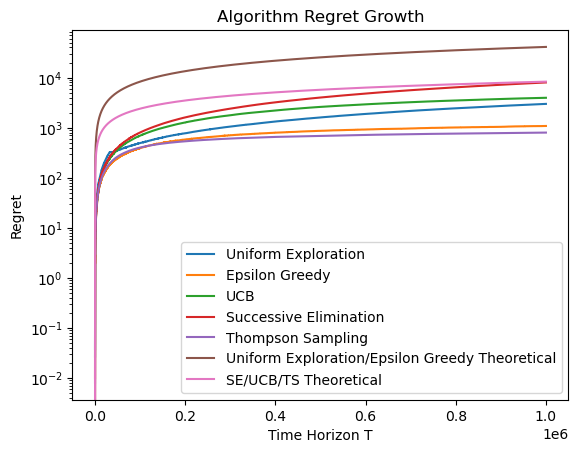
\includegraphics[width=0.7\textwidth]{allregret.png}
    \caption{Cumulative regret over time.}
    \label{fig:regret}
\end{figure}

From the regret plot as shown in Figure~\ref{fig:regret}, there are two main points to take away from this simulation. First, each algorithm incurs less regrets regret than their corresponding theoretical upper bounds. This is expected since these bounds are worst-case guarantees and are generally not tight for specific problem instances. The second observation is that the algorithms exhibit a clear ordering in performance, with Thompson Sampling achieving the lowest regret, followed by Successive Elimination, while Uniform Exploration performs the worst. This ordering can be explained by how efficiently each algorithm allocates its samples. Uniform Exploration continues to sample all arms equally, including clearly suboptimal ones, resulting in many wasted pulls. Successive Elimination improves upon this by progressively discarding arms that appear suboptimal, thereby concentrating more samples on promising arms. Thompson Sampling is even more efficient, allocating pulls according to the posterior probability that each arm is optimal. As a result, it focuses exploration on uncertain but potentially optimal arms while rapidly exploiting strong candidates. This increasingly efficient allocation of samples leads to progressively lower cumulative regret. 

Overall, this simulation provides an empirical complement to the theoretical results established earlier. In particular, it illustrates that the regret bounds derived for each algorithm are not only theoretically meaningful but also reflect their practical performance. Moreover, the observed ordering of algorithms is consistent with their theoretical guarantees, with more adaptive methods achieving lower regret in practice

\section{Conclusion}

Overall, in this report, we studied multi-armed bandit problems and analysed the performance of several classical algorithms, including Uniform Exploration, Successive Elimination, and Thompson Sampling. We derived regret upper bounds for each algorithm and showed that adaptive strategies achieve significantly improved performance compared to non-adaptive exploration. We further established a fundamental lower bound of order $\Omega(\sqrt{KT})$ on the expected regret, showing that no algorithm can avoid the exploration–exploitation trade-off in the worst case. Our numerical experiments supported the theoretical findings, illustrating both the relative performance of the algorithms and the gap between worst-case guarantees and typical instance behaviour. The framework analysed and established here provides a foundation for many real world applications such as in reinforcement learning, sequential portfolio selection, online advertising, dynamic pricing etc \cite{DBLP:journals/corr/abs-1904-10040}


\section{Limitations and Future Work}

There are a few areas of this current multi-armed bandit model which can be extended and further studied. 

First, is the relaxation of the assumption that the rewards for these bandit problems need to be fixed over the whole time horizon. Instead rewards can change over time and therefore a different model is needed. This leads to research into non-stationary bandit models and algorithms based on discounted rewards or sliding-window estimates, which place greater emphasis on recent observations and can adapt to changing environments \cite{zhou2025bandits}. 

Furthermore, Our current bandit model assumes we can only make decisions solely on the basis of previous rewards. Further research can look into relaxing this restriction by exploring bandit problems where there is side information available before each decision called contextual bandits \cite{DBLP:journals/corr/abs-1807-09809}. 

Finally, another area of further research is to study multi-armed bandits from a dynamic programming perspective, where the objective is to characterise optimal policies, for example via the Gittins index \cite{scully2025gittinsindexdesignprinciple}, rather than focusing solely on asymptotic regret guarantees.

\newpage

\printbibliography


\end{document}